\documentclass{standalone}
\usepackage{tikz}
\usetikzlibrary{patterns, positioning}


\begin{document}
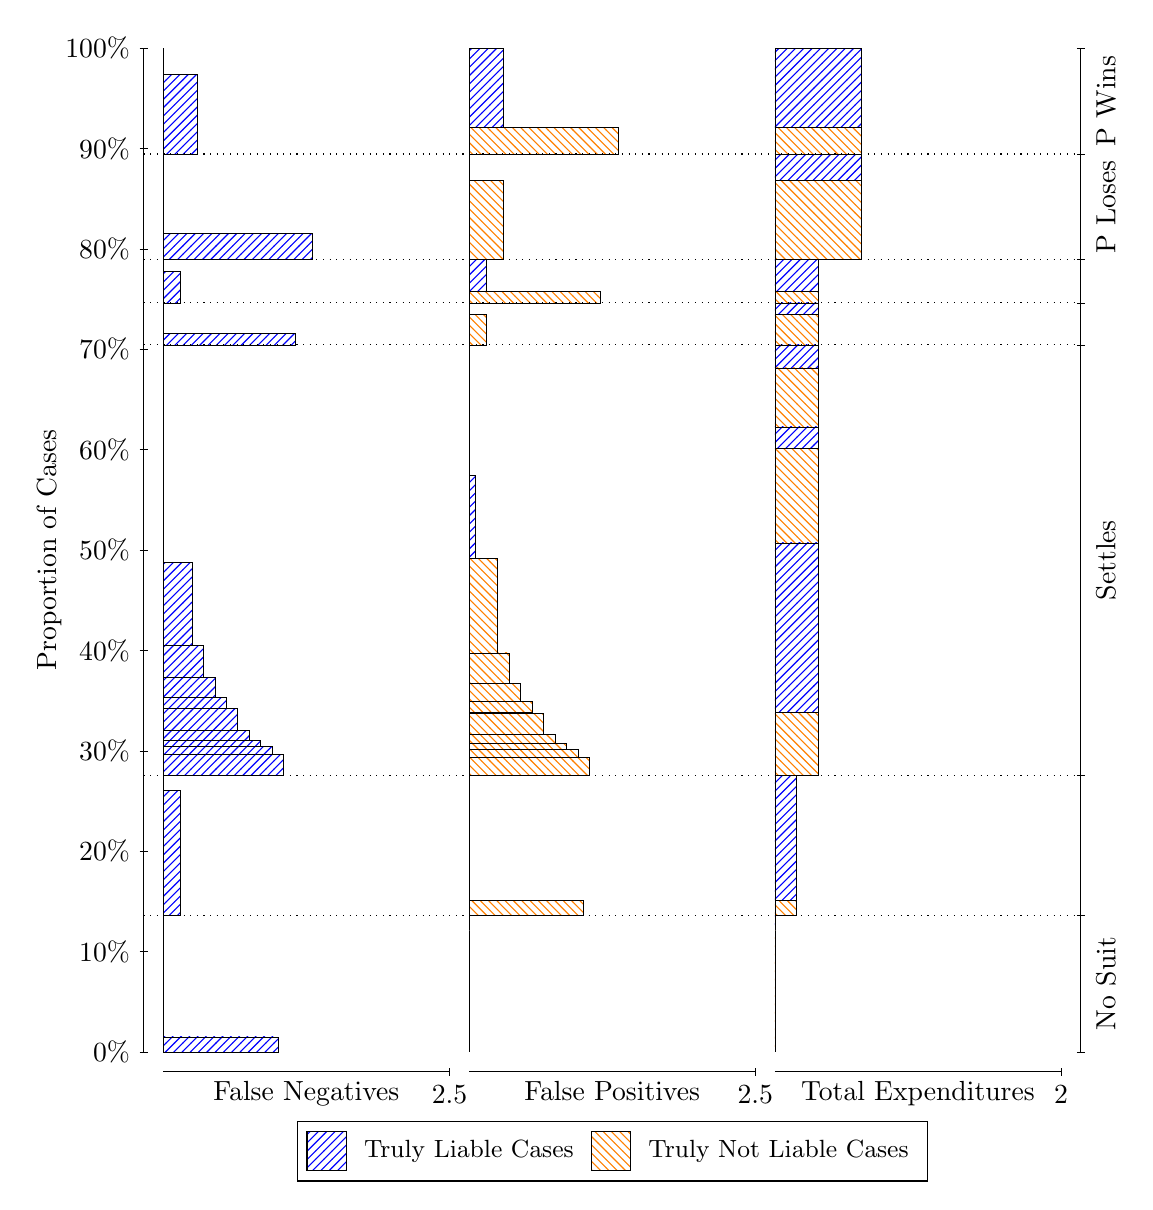
\begin{tikzpicture}
\draw[black, very thin] (1.5,1.75) -- (1.5,14.5);
\node[rotate=90, text=black, anchor=center] at (0.3, 8.125) {Proportion of Cases};
\draw[black, very thin] (1.45,1.75) -- (1.55,1.75);
\node[text=black, anchor=east] at (1.45, 1.75) {0\%};
\draw[black, very thin] (1.45,3.025) -- (1.55,3.025);
\node[text=black, anchor=east] at (1.45, 3.025) {10\%};
\draw[black, very thin] (1.45,4.3) -- (1.55,4.3);
\node[text=black, anchor=east] at (1.45, 4.3) {20\%};
\draw[black, very thin] (1.45,5.575) -- (1.55,5.575);
\node[text=black, anchor=east] at (1.45, 5.575) {30\%};
\draw[black, very thin] (1.45,6.85) -- (1.55,6.85);
\node[text=black, anchor=east] at (1.45, 6.85) {40\%};
\draw[black, very thin] (1.45,8.125) -- (1.55,8.125);
\node[text=black, anchor=east] at (1.45, 8.125) {50\%};
\draw[black, very thin] (1.45,9.4) -- (1.55,9.4);
\node[text=black, anchor=east] at (1.45, 9.4) {60\%};
\draw[black, very thin] (1.45,10.675) -- (1.55,10.675);
\node[text=black, anchor=east] at (1.45, 10.675) {70\%};
\draw[black, very thin] (1.45,11.95) -- (1.55,11.95);
\node[text=black, anchor=east] at (1.45, 11.95) {80\%};
\draw[black, very thin] (1.45,13.225) -- (1.55,13.225);
\node[text=black, anchor=east] at (1.45, 13.225) {90\%};
\draw[black, very thin] (1.45,14.5) -- (1.55,14.5);
\node[text=black, anchor=east] at (1.45, 14.5) {100\%};

\draw[black, very thin] (13.4,1.75) -- (13.4,14.5);
\draw[black, very thin] (13.35,1.75) -- (13.45,1.75);
\node[anchor=west] at (13.35, 1.75) {};
\draw[black, very thin] (13.35,3.4862) -- (13.45,3.4862);
\node[anchor=west] at (13.35, 3.4862) {};
\draw[black, very thin] (13.35,5.2624) -- (13.45,5.2624);
\node[anchor=west] at (13.35, 5.2624) {};
\draw[black, very thin] (13.35,10.73) -- (13.45,10.73);
\node[anchor=west] at (13.35, 10.73) {};
\draw[black, very thin] (13.35,11.263) -- (13.45,11.263);
\node[anchor=west] at (13.35, 11.263) {};
\draw[black, very thin] (13.35,11.811) -- (13.45,11.811);
\node[anchor=west] at (13.35, 11.811) {};
\draw[black, very thin] (13.35,13.154) -- (13.45,13.154);
\node[anchor=west] at (13.35, 13.154) {};
\draw[black, very thin] (13.35,14.5) -- (13.45,14.5);
\node[anchor=west] at (13.35, 14.5) {};

\draw[black, very thin, pattern color=blue, pattern=north east lines] (1.75,1.75) rectangle (3.2033,1.9405);
\draw[black, very thin, pattern color=orange, pattern=north west lines] (1.75,1.9405) rectangle (1.75,3.4862);
\draw[black, very thin, pattern color=blue, pattern=north east lines] (1.75,3.4862) rectangle (1.968,5.0719);
\draw[black, very thin, pattern color=orange, pattern=north west lines] (1.75,5.0719) rectangle (1.75,5.2624);
\draw[black, very thin, pattern color=blue, pattern=north east lines] (1.75,5.2624) rectangle (3.276,5.5334);
\draw[black, very thin, pattern color=blue, pattern=north east lines] (1.75,5.5334) rectangle (3.1307,5.6314);
\draw[black, very thin, pattern color=blue, pattern=north east lines] (1.75,5.6314) rectangle (2.9853,5.707);
\draw[black, very thin, pattern color=blue, pattern=north east lines] (1.75,5.707) rectangle (2.84,5.8376);
\draw[black, very thin, pattern color=blue, pattern=north east lines] (1.75,5.8376) rectangle (2.6947,6.1113);
\draw[black, very thin, pattern color=blue, pattern=north east lines] (1.75,6.1113) rectangle (2.5493,6.2532);
\draw[black, very thin, pattern color=blue, pattern=north east lines] (1.75,6.2532) rectangle (2.404,6.5073);
\draw[black, very thin, pattern color=blue, pattern=north east lines] (1.75,6.5073) rectangle (2.2587,6.9163);
\draw[black, very thin, pattern color=blue, pattern=north east lines] (1.75,6.9163) rectangle (2.1133,7.9726);
\draw[black, very thin, pattern color=orange, pattern=north west lines] (1.75,7.9726) rectangle (1.75,10.73);
\draw[black, very thin, pattern color=blue, pattern=north east lines] (1.75,10.73) rectangle (3.4213,10.875);
\draw[black, very thin, pattern color=orange, pattern=north west lines] (1.75,10.875) rectangle (1.75,11.263);
\draw[black, very thin, pattern color=blue, pattern=north east lines] (1.75,11.263) rectangle (1.968,11.66);
\draw[black, very thin, pattern color=orange, pattern=north west lines] (1.75,11.66) rectangle (1.75,11.811);
\draw[black, very thin, pattern color=blue, pattern=north east lines] (1.75,11.811) rectangle (3.6393,12.147);
\draw[black, very thin, pattern color=orange, pattern=north west lines] (1.75,12.147) rectangle (1.75,13.154);
\draw[black, very thin, pattern color=blue, pattern=north east lines] (1.75,13.154) rectangle (2.186,14.164);
\draw[black, very thin, pattern color=orange, pattern=north west lines] (1.75,14.164) rectangle (1.75,14.5);
\draw[black, very thin, pattern color=orange, pattern=north west lines] (5.6333,1.75) rectangle (5.6333,3.2957);
\draw[black, very thin, pattern color=blue, pattern=north east lines] (5.6333,3.2957) rectangle (5.6333,3.4862);
\draw[black, very thin, pattern color=orange, pattern=north west lines] (5.6333,3.4862) rectangle (7.0867,3.6767);
\draw[black, very thin, pattern color=blue, pattern=north east lines] (5.6333,3.6767) rectangle (5.6333,5.2624);
\draw[black, very thin, pattern color=orange, pattern=north west lines] (5.6333,5.2624) rectangle (7.1593,5.4951);
\draw[black, very thin, pattern color=orange, pattern=north west lines] (5.6333,5.4951) rectangle (7.014,5.591);
\draw[black, very thin, pattern color=orange, pattern=north west lines] (5.6333,5.591) rectangle (6.8687,5.6693);
\draw[black, very thin, pattern color=orange, pattern=north west lines] (5.6333,5.6693) rectangle (6.7233,5.7852);
\draw[black, very thin, pattern color=orange, pattern=north west lines] (5.6333,5.7852) rectangle (6.578,6.0526);
\draw[black, very thin, pattern color=orange, pattern=north west lines] (5.6333,6.0526) rectangle (6.4327,6.0673);
\draw[black, very thin, pattern color=orange, pattern=north west lines] (5.6333,6.0673) rectangle (6.4327,6.2053);
\draw[black, very thin, pattern color=orange, pattern=north west lines] (5.6333,6.2053) rectangle (6.2873,6.4292);
\draw[black, very thin, pattern color=orange, pattern=north west lines] (5.6333,6.4292) rectangle (6.142,6.819);
\draw[black, very thin, pattern color=orange, pattern=north west lines] (5.6333,6.819) rectangle (5.9967,8.0199);
\draw[black, very thin, pattern color=blue, pattern=north east lines] (5.6333,8.0199) rectangle (5.706,9.0763);
\draw[black, very thin, pattern color=blue, pattern=north east lines] (5.6333,9.0763) rectangle (5.6333,10.73);
\draw[black, very thin, pattern color=orange, pattern=north west lines] (5.6333,10.73) rectangle (5.8513,11.118);
\draw[black, very thin, pattern color=blue, pattern=north east lines] (5.6333,11.118) rectangle (5.6333,11.263);
\draw[black, very thin, pattern color=orange, pattern=north west lines] (5.6333,11.263) rectangle (7.3047,11.413);
\draw[black, very thin, pattern color=blue, pattern=north east lines] (5.6333,11.413) rectangle (5.8513,11.811);
\draw[black, very thin, pattern color=orange, pattern=north west lines] (5.6333,11.811) rectangle (6.0693,12.818);
\draw[black, very thin, pattern color=blue, pattern=north east lines] (5.6333,12.818) rectangle (5.6333,13.154);
\draw[black, very thin, pattern color=orange, pattern=north west lines] (5.6333,13.154) rectangle (7.5227,13.49);
\draw[black, very thin, pattern color=blue, pattern=north east lines] (5.6333,13.49) rectangle (6.0693,14.5);
\draw[black, very thin, pattern color=orange, pattern=north west lines] (9.5167,1.75) rectangle (9.5167,3.2957);
\draw[black, very thin, pattern color=blue, pattern=north east lines] (9.5167,3.2957) rectangle (9.5167,3.4862);
\draw[black, very thin, pattern color=orange, pattern=north west lines] (9.5167,3.4862) rectangle (9.7892,3.6767);
\draw[black, very thin, pattern color=blue, pattern=north east lines] (9.5167,3.6767) rectangle (9.7892,5.2624);
\draw[black, very thin, pattern color=orange, pattern=north west lines] (9.5167,5.2624) rectangle (10.062,6.0673);
\draw[black, very thin, pattern color=blue, pattern=north east lines] (9.5167,6.0673) rectangle (10.062,8.2153);
\draw[black, very thin, pattern color=orange, pattern=north west lines] (9.5167,8.2153) rectangle (10.062,9.4162);
\draw[black, very thin, pattern color=blue, pattern=north east lines] (9.5167,9.4162) rectangle (10.062,9.6872);
\draw[black, very thin, pattern color=orange, pattern=north west lines] (9.5167,9.6872) rectangle (10.062,10.439);
\draw[black, very thin, pattern color=blue, pattern=north east lines] (9.5167,10.439) rectangle (10.062,10.73);
\draw[black, very thin, pattern color=orange, pattern=north west lines] (9.5167,10.73) rectangle (10.062,11.118);
\draw[black, very thin, pattern color=blue, pattern=north east lines] (9.5167,11.118) rectangle (10.062,11.263);
\draw[black, very thin, pattern color=orange, pattern=north west lines] (9.5167,11.263) rectangle (10.062,11.413);
\draw[black, very thin, pattern color=blue, pattern=north east lines] (9.5167,11.413) rectangle (10.062,11.811);
\draw[black, very thin, pattern color=orange, pattern=north west lines] (9.5167,11.811) rectangle (10.607,12.818);
\draw[black, very thin, pattern color=blue, pattern=north east lines] (9.5167,12.818) rectangle (10.607,13.154);
\draw[black, very thin, pattern color=orange, pattern=north west lines] (9.5167,13.154) rectangle (10.607,13.49);
\draw[black, very thin, pattern color=blue, pattern=north east lines] (9.5167,13.49) rectangle (10.607,14.5);
\draw[black, dotted] (1.5,3.4862) -- (13.4,3.4862);
\draw[black, dotted] (1.5,5.2624) -- (13.4,5.2624);
\draw[black, dotted] (1.5,10.73) -- (13.4,10.73);
\draw[black, dotted] (1.5,11.263) -- (13.4,11.263);
\draw[black, dotted] (1.5,11.811) -- (13.4,11.811);
\draw[black, dotted] (1.5,13.154) -- (13.4,13.154);
\draw[black, very thin] (1.75,1.5) -- (5.3833,1.5);
\node[text=black, anchor=north] at (3.5667, 1.5) {False Negatives};
\draw[black, very thin] (5.3833,1.45) -- (5.3833,1.55);
\node[text=black, anchor=north] at (5.3833, 1.45) {2.5};

\draw[black, very thin] (5.6333,1.5) -- (9.2667,1.5);
\node[text=black, anchor=north] at (7.45, 1.5) {False Positives};
\draw[black, very thin] (9.2667,1.45) -- (9.2667,1.55);
\node[text=black, anchor=north] at (9.2667, 1.45) {2.5};

\draw[black, very thin] (9.5167,1.5) -- (13.15,1.5);
\node[text=black, anchor=north] at (11.333, 1.5) {Total Expenditures};
\draw[black, very thin] (13.15,1.45) -- (13.15,1.55);
\node[text=black, anchor=north] at (13.15, 1.45) {2};

\node[text=black, centered, rotate=90] at (13.72, 2.6181) {No Suit};

\node[text=black, centered, rotate=90] at (13.72, 7.9963) {Settles};


\node[text=black, centered, rotate=90] at (13.72, 12.483) {P Loses};
\node[text=black, centered, rotate=90] at (13.72, 13.827) {P Wins};

\draw (7.449999999999999,1.5) node[draw=none] (baseCoordinate) {};
\begin{scope}[align=center]
        \matrix[scale=0.5, draw=black, below=0.5cm of baseCoordinate, nodes={draw}, column sep=0.1cm]{
            \node[rectangle, draw, minimum width=0.5cm, minimum height=0.5cm, pattern color=blue, pattern=north east lines] {}; &
            \node[draw=none, font=\small, text=black] (B) {Truly Liable Cases}; &
            \node[rectangle, draw, minimum width=0.5cm, minimum height=0.5cm, pattern color=orange, pattern=north west lines] {}; &
            \node[draw=none, font=\small, text=black] (B) {Truly Not Liable Cases}; \\
            };
\end{scope}

\end{tikzpicture}
\end{document}